

\subsection{Proposed validation}

In this chapter, we discuss our approach to validate the proposed method and compare it with existing methods with some benchmarking data sets. The competitive methods are ORA, Kolmogorov-Smirnov test, Wilcoxon, FGSEA, and IPA. We describe 16 data sets from three species, namely human, mouse, and rat, with 8 different CDTs used for methods comparison. %Out of these 16 data sets, 14 data sets are used for testing the hypothesis 1, and the other two are used for validating the hypothesis 2.

\subsubsection{Benchmarking methods}
%\subsubsection{}

The ORA family of methods, as well as other tests, such as KS, Wilcoxon, and FGSEA, are widely used in gene set analysis to determine whether  a particular gene set - such as the genes associated to a given GO term or pathway - is significantly affected in the given phenotype. In principle, the same approach could be used to decide whether a given CDT could be related to the phenotype by considering the set of genes known to be affected by the given CDT. 

\textbf{ORA} uses a statistical test, such as hypergeometric, chi-square, or binomial distribution, to evaluate if the number of DE genes is over- or under-represented in the set of targeted genes of a CDT. In this study, we would use hypergeometric test to compute p value, namely the probability of getting the $x$ or more observed DE genes in $M$ CDT's downstream genes from a pool of $N$ background genes with $n$ DE genes. Mathematically, this probability is defined as:

\begin{equation*}
P(X \geq x) = 1-P(X \leq x -1)= 1- \sum_{i=0}^{x-1} \frac{\binom{M}{i}\binom{N-M}{n-i}}{\binom{N}{n}} 
\end{equation*}

ORA does not take into consideration if the DE gene is up-regulated or down-regulated, nor the type of associations between the CDT and the targeted DE gene.

The Kolmogorov-Smirnov test (\textbf{KS}) determines whether there is a significantly difference between two empirical distributions of the scores (the direction of the fold changes) of the DE genes targeted by the CDT (\texttt{DEhit}) and those of the DE genes not targeted by the CDT (\texttt{DEmiss}). First, all genes will be ranked in order of their log fold changes. Then, we calculate the cumulative distribution function (CDF) of the ranked gene list for background genes and for the genes affected by the CDT. Finally, the KS test is used to compare the two CDFs and calculates a p value that measures the significance of the enrichment. Although KS takes the sign of the DE genes into consideration (the fold changes of gene expression), it ignores the type of associations between CDTs and DE genes.

\textbf{Wilcoxon} is a rank-based non-parametric test for comparing the ranks of DE genes affected by the CDT (\texttt{DEhit}), and other DE genes (\texttt{DEmiss}). First, it ranks all genes in both lists based on their fold changes. Subsequently, it computes the a test statistic $W$, which is the sum of the ranks for all \texttt{DEhit}. This test statistic $W$ is compared to the distribution of $W$ under the null hypothesis. The null hypothesis is rejected if $W$ is extreme and falls outside 95\% of the distribution. In R, the Wilcoxon is available via the function \texttt{wilcox.test}.  Similar to ORA, the  associations of the affected DE genes with the CDT are completely ignored.

\textbf{FGSEA} is an improvement of the Gene Set Enrichment Analysis (GSEA) approach. FGSEA accelerates the calculation of the GSEA p value by estimating it with a high accuracy (the estimation error is less than $10^{-100}$ when compared with actual GSEA p value). GSEA, in turn, is one of the most popular approaches in gene set analysis\cite{Subramanian:2005}. It consists of three important steps: computing the enrichment score for each gene set, estimating the statistical significance of the enrichment score, and adjusting for multiple hypothesis testing. We used the function \texttt{fgsea} in the ``fgsea'' package with the parameters \texttt{nperm = 10\textsuperscript{4}} and \texttt{minSize = 15}.

\textbf{IPA} is a commercial web-based platform that offers several applications including a causal analysis tool\cite{kramer2013causal}. Given a list of DE genes, IPA's causal analysis outputs a list of upstream regulators including chemicals/drugs, as well as genes, proteins families, complexes, microRNA, and biological processes.
Notice that including all these types of regulators in the report would worsen the IPA's result when benchmarking with other methods since it might increase the rank of the true CDT. Moreover, since there is only one true causal CDT in each experiment and all other elements are considered as false positives, having them in the result would increase the number of false positives. 
For these reasons, beside the default IPA result, we added to the method benchmarking the so-called IPA-CDT  that only retains the CDTs in the IPA report and excludes all non-chemical elements.

According to Kr\"{a}mer \textit{et al.}, IPA derives two scores for each regulator \textit{r}, namely the overlap p-value and the activation z-score, as follows.

\emph{The overlap p-value} reflects the enrichment of the list of \textit{r}-regulated genes in the set of all DE genes without taking the regulation direction into consideration. Formally, it is based on the one-sided Fisher's exact test and is calculated as follows:

\begin{equation*}
p(r)=\sum_{k = 0}^{min(c,d)} \frac{(a+b)!(c+d)!(a+c)!(b+d)!}{(a+k)!(b-k)!(c-k)!(d+k)!n!}
\end{equation*}

where $n$ is the number of all background genes, i.e. all the genes in the data set that have at least one association with any upstream regulator, $a$ is the number of DE genes regulated by $r$, $b$ is the number of DE genes that are not regulated by $r$, $c$ is the number of $r$-regulated genes but not differentially expressed, and $d=n-a-b-c$.

\emph{The activation z-score} uses the information about the direction of gene regulation to predict the regulators. Let $\tilde{O}$ be the set of $r$-regulated DE genes, the activation z-score of the corresponding regulator $r$ is defined as:


\begin{equation*}
z(r) =  \frac{\sum\limits_{v \in \tilde{O}}w_{R}(r,v) s_{R}(r,v) s_{D}(v)}{\left(\sum\limits_{v \in \tilde{O}}[w_{R}(r,v)]^2\right)^{1/2}}
\end{equation*}

where $w_{R}(r,v)$ represents the weight associated with the regulation of $r$ and the downstream DE gene $v$, $s_{R}(r,v)$ is the sign of the regulation, i.e. $s_{R}(r,v)=1$ for activation and $s_{R}(r,v)=-1$ for inhibition, and $s_{D}(v)$ represents the direction of DE gene's expression, i.e. $s_{D}(v)=1$ for up-regulation and $s_{D}(v)=-1$ for down-regulation, respectively. The activation z-score is proven to be approximately normally distributed under the null model, e.g. random signs $s_{R}(r,v)$ and $s_{D}(v)$. On one hand, a high positive z-score, e.g. $z(r) > 2$, indicates that the match between the signs of downstream DE genes ($s_{D}(v)$) and the corresponding edges ($s_{R}(r,v)$) is significant, which in turn suggests that $r$ is the activated regulator. On the other hand, a low negative z-score, e.g. $z(r) <  -2$, is an indicator that the sign of the downstream DE genes are mostly opposite with the corresponding regulations. In this case, $r$ is predicted as an inhibitor~\cite{kramer2013causal}.




\subsubsection{Validation data sets}

We downloaded 16 benchmark data sets from Gene Expression Omnibus database (GEO: \url{https://www.ncbi.nlm.nih.gov/geo/}). 
%These data sets are experiments in which gene expressions of control samples are compared with samples exposed to a studied CDT. 
These experiments varied from human, mouse, to rat with 8 different CDTs (See Table~\ref{Datasets}).

The DE genes are selected using a threshold of $|log(FC)| > 0.6$ and $p\ value < 0.05$.

Out of these 16 data sets, the first 14 data sets are used for testing the hypothesis 1, and the other two are used for validating the hypothesis 2.


\begin{table}
\caption{The detailed information of 16 benchmarking data sets used in this manuscript. All data sets are downloaded from Gene Expression Omnibus (GEO) database.}
\label{Datasets} 
\begin{center}
\scriptsize
\begin{tabular}{ c|cccc } 

 \hline \hline
Experiment ID & GEO ID& Organism& True CDT  &Hypothesis\\ 
\hline
1  & GSE26487~\cite{stojadinovic2007novel}& Human & Dexamethasone & H1 \\ 
2  & GSE49804~\cite{peffer2014caveolin}& Mouse & Dexamethasone & H1\\ 
3  & GSE86837~\cite{stenz2017testicular}& Mouse & Diethylhexyl Phthalate &H1\\ 
4  & GSE58434\_H~\cite{himes2015vitamin}$^{(1)}$& Human & Calcitriol (Vitamin D) &H1\\ 
5  & GSE58434\_Ast~\cite{himes2015vitamin}$^{(2)}$& Human & Calcitriol (Vitamin D)  &H1\\ 
6  & GSE11352\_12h~\cite{lin2007whole} & Human & Estradiol  &H1\\ 
7  & GSE11352\_24h~\cite{lin2007whole}& Human & Estradiol &H1 \\ 
8  & GSE11352\_48h~\cite{lin2007whole} & Human & Estradiol &H1\\ 
9  & GSE74000~\cite{rodrigues2016gene} & Human & Acetaminophen &H1\\ 
10 & GSE12446~\cite{Hanifi-Moghaddam:2007} & Human & Estradiol &H1\\
11 & GSE67266\_WT$^{(3)}$	& Mouse	& Etoposide &H1\\
12 & GSE67266\_KO$^{(4)}$ &	Mouse &	Etoposide &H1 \\
13 & GSE51213	& Mouse	& Dexamethasone&H1\\
14 & GSE58875~\cite{tallino2015nutrigenomics}	& Rat & Copper deficiency &H1\\
15 & GSE147507\_NHBE~\cite{Blanco-Melo:2020}$^{(5)}$ & Human & Methylprednisolone&H2\\
16 & GSE147507\_A549~\cite{Blanco-Melo:2020}$^{(6)}$ & Human & Methylprednisolone&H2\\
 \hline\hline
 \multicolumn{5}{l}{\tiny $^{(1)}$ Contrast: Healthy patient treated with vitamin D vs healthy patient untreated}\\
 \multicolumn{5}{l}{\tiny $^{(2)}$ Contrast: Asthma patient treated with vitamin D vs asthma patient untreated}\\
 \multicolumn{5}{l}{\tiny $^{(3)}$ Contrast: Wild Type (WT) mice treated with etoposide vs mock treated after 6 hours}\\
 \multicolumn{5}{l}{\tiny $^{(4)}$ Contrast: MK2/3 knockout (KO) mice treated with etoposide vs mock treated after 6 hours}\\
 \multicolumn{5}{l}{\tiny $^{(5)}$ Contrast: Primary normal human bronchial epithelial cells (NHBE) infected with COVID-19 vs control}\\
 \multicolumn{5}{l}{\tiny $^{(6)}$ Contrast: A549 lung cell line infected with COVID-19 versus control}\\
\end{tabular}
\end{center}
\end{table}


\subsubsection{Assessment criteria}

%\subsubsection{Assessment}

We would evaluate and compare the performance of our proposed method with the other five approaches, namely Over Representation Analysis (ORA) using hypergeometric test, Kolmogorov-Smirnov test (KS)\cite{massey1951kolmogorov}, Wilcoxon\cite{wilcoxon1945individual}, FGSEA~\cite{korotkevich2021fast}, and the causal analysis used in Ingenuity Pathway Analysis (IPA)~\cite{kramer2013causal}.



\textbf{Assessment of hypothesis 1}

We would evaluate these methods using 14 benchmark data sets from three different species, namely human, mouse, and rat (See Table \ref{Datasets}, experiment ID from 1 - 14). 
In these data sets, gene expressions were measured after the ingestion of a given CDT.
Hence, the cause of all the changes observed  throughout the system is known. Furthermore, this particular situation corresponds to  H1, where the level of the CDT is higher than normal.
We consider the administered CDT as the ``true CDT'' for each of these data sets.

The result of each method is a ranked list of CDTs based on the particular statistic used by each method, i.e. FDR-adjusted p values for our proposed method, ORA, KS, Wilcoxon, and FGSEA, and  z-score  for IPA and IPA-CDT. 
If several CDTs are ranked with the same statistic, we use an average. For instance, if  the top 4 elements have the same p value, they would be all ranked as 2.5 instead of 1, 2, 3, and 4, respectively because 2.5 is the average of the set $\{1, 2, 3, 4\}$.
An ideal method would be able to identify the true CDT by ranking it on top with a significant p value $\leq 0.05$ or  z-score $\geq 2$ (or z-score $\leq -2$ in case of IPA testing the H2).

%There are 14 data sets corresponding to the H1 where the causal CDTs are known (Table~\ref{Datasets}). We report and compare the ranks of the true CDTs in these 14 data sets (see Table~\ref{Ranks} and Fig.~\ref{fig:resultFigure}a).
%PURE (average = 2.8) is better than all of the methods in this study, followed by IPA-CDT (average = 17.7), ORA (average = 20.1), and KS (average = 24), GSEA (average = 32.9), IPA (average = 79.9), and Wilcoxon (average = 104.4) (Table \ref{Ranks}). PURE can successfully identify the true CDTs in these 14 benchmarking data sets and rank them at the top 7 times. It performs better than all of the methods in 9 data sets. IPA-CDT performs best in 6 data sets (3 of which are tied with PURE) and is able to rank the true CDTs at the top 5 times. However, it cannot identify the true CDTs in three data sets, in two of which the true CDTs are not present in the result list (data set 8 and data set 14). Similar to IPA-CDT, IPA can correctly rank the true CDTs at the top in 5 data sets.  FGSEA performs best in 2 data sets. ORA performs best in one data sets (tied with PURE), while KS and Wilcoxon are not able to perform best in any of the experiment.


Notice that an evaluation based solely on the method's ability to identify the true CDT using the p value does not show the whole story and sometimes misleads.
For example, a method that derives low p values for all CDTs can always identify the true CDT, but is still considered a bad one because it includes a lot of false positives in the result.
Therefore, we would also take the number of false positives in the result into consideration, i.e. the number of CDTs that are not true CDT but reported as significant. % (Fig. \ref{fig:resultFigure}b).
Although chemicals and drugs could have similar effects or could be in the same family, we only consider the true CDT as the one and only true positive and all other CDTs as true negatives.
We expect a good method would derive a low number of CDTs in the result, ideally only one, the true CDT.
%Our method generally reports the lower numbers of reported chemicals (average = 19.4) than any other methods compared, followed by FGSEA (average = 37.4) and IPA-CDT (average = 37.6).
%Although FGSEA is comparable to IPA-CDT, it cannot identify the true CDTs in 6 out of 14 experiments while IPA  cannot identify only 3 out of 15.
%Wilcoxon and IPA report on average more than 100 CDTs while ORA and KS report on average more than 200 CDTs per experiment (Table \ref{NrSig}).


%e.g in the experiment 9 performed by IPA, we assigned 31 to the true CDT's rank because IPA reported a list of 30 significant CDTs but the true CDTs is not included (Table ~\ref{NrSig}). 
%The p value for the number of CDTs reported comparison between PURE and IPA-CDT, ORA, KS,  FGSEA, IPA, and Wilcoxon are 0.04, 4E-4, 9E-6, 0.4, 4E-5, and 2E-6, respectively. 
%Since all  p values are less than the standard threshold of 0.05 (except for FGSEA while comparing the number of CDTs reported), PURE's performance can be considered significantly better than all of the methods included in the study, in terms of both the rank of the true CDTs, as well as the number of significant CDTs reported.

\textbf{Assessment of hypothesis 2}

The assessment of these methods on testing H2 is more challenging since the data sets in which the ground truth is known are scant, i.e. an CDT is truly lacking in the system. Another important application for testing the H2 is drug repurposing. A CDT could potentially reverse the  gene expression changes caused by the disease and therefore be a candidate for drug repurposing. 
%Similar approach using the data set GSE147507, in which the expression of NHBE and A549 cells infected with COVID-19 were compared with their corresponding control, proposed Methylprednisolone to improve the outcome in server COVID-19 cases~\cite{DraghiciCOVID:2021}. This finding was aligned with several clinical trials from different research groups~\cite{DraghiciCOVID:2021, corral2021methylprednisolone,salton2020prolonged, meduri2020pharmacological}. 
%At the time we applied PURE to the COVID-19 data, the recommendation of several organizations, including the World Health Organization (WHO), CDC, and Surviving Sepsis Campaign, was against the use of any systemic corticosteroids in the severe cases of COVID-19~\cite{wilson2020covid}. 
%Surprisingly, our results showed that Methylprednisolone, a corticosteroid, would be effective in helping the patients with severe disease~\cite{DraghiciCOVID:2021}. 


During COVID-19 pandemic in 2020,  researchers around the world were focusing to find a drug that treats the COVID-19. For the short period of time, the popular and feasible approach at the time was drug repurposing. Clinical trials have shown that  steroids are effective \cite{meduri2020pharmacological, corral2021methylprednisolone,salton2020prolonged, meduri2020pharmacological, cochrane1996systemic, prescott2020corticosteroids}, and the World Health Organization (WHO) has reversed their previous recommendation against the use of any systemic corticosteroids in the severe cases of COVID-19~\cite{wilson2020covid}. At this time, the standard of care in severe cases of COVID-19 is the corticosteroid treatment. 
Hence, in this study, we would use the data set GSE147507 in which the expression of NHBE and A549 cells infected with COVID-19 were compared with their corresponding control, and consider Methylprednisolone as the ``target'' CDT in the experiments 15 and 16 for different contrasts. %(Table~\ref{H2Result}).

Similarly to testing the H1, we would validate whether a method can identify the target CDT and has as few false positives as possible.
%PURE can identify the true CDTs in all of the experiments.
%Also notice that in data set 13, IPA could determine the target chemical, dexamethasone, as significant and rank it 13, there are 173 other false positive chemicals in the result.
%

%
%\begin{table}
%\caption{\label{Ranks} Benchmarking the methods in term of the ranks of the true CDTs. The experiment IDs (Exp. ID) are corresponding to the ones in Table \ref{Datasets}. The lower the rank of the true CDTs, the better.  The green highlighted cell is the best one in each experiment. PURE performs best in 9 out of 14 experiments, followed by IPA which performs best in 6 experiments (3 co-best with PURE). In two of the data sets analyzed IPA was not able to identify the correct CDT at all  (highlighted in red).}
%\begin{center}
%\scriptsize
%\begin{tabular}{ ccc|ccccccc } 
%
% \hline \hline
%
%\multirow{2}{*}{Exp. ID}& \multirow{2}{*}{GEO ID}& \multirow{2}{*}{Organism} & \multicolumn{7}{c}{\textbf{Rank of true CDTs}} \\
%&  && PURE  & ORA & KS  & Wilcoxon & FGSEA & IPA& IPA-CDT\\
%\hline
%1	& GSE26487& Human &	\cellcolor{green}1	&	1.5	&	43	&	45	&	25.5	& \cellcolor{green}1&	\cellcolor{green}1\\ 
%
%2	& GSE49804& Mouse	&	2	&	2	&	33	&	11	&	16.5	&	\cellcolor{green}1 & \cellcolor{green}1\\ 
%
%3	& GSE86837& Mouse	&	\cellcolor{green}1	&	\cellcolor{green}1	&	3	&	2.5	&	47	&	816& 153\\ 
%
%4	& GSE58434\_H& Human &	\cellcolor{green}1	&	16	&	13.5	&	65	&	159	&	25 & 14\\ 
%
%5	& GSE58434\_Ast& Human &	\cellcolor{green}2	&	18	&	23.5	&	254	&	30.5	&	26 & 5\\ 
%
%6	& GSE11352\_12h & Human	&	\cellcolor{green}1	&	32.5	&	24.5	&	126	&	4.5	&	\cellcolor{green}1 & \cellcolor{green}1\\ 
%
%7	& GSE11352\_24h & Human	&	\cellcolor{green}1	&	33	&	24	&	214	&	7.5	&	\cellcolor{green}1 & \cellcolor{green}1\\ 
%
%8	& GSE11352\_48h & Human	&	2	&	29.5	&	24	&	153	&	24.5	&	\cellcolor{green}1 & \cellcolor{green}1\\ 
%
%9	& GSE74000 & Human	&	\cellcolor{green}1	&	16	&	23	&	9	&	75	&	\cellcolor{red}NA & \cellcolor{red}NA\\ 
%
%10	& GSE12446\_WT & Human	&	4	&	31	&	39.5	&	460.5	&	27.5	& 10 & 	\cellcolor{green}3\\ 
%
%11	& GSE67266\_KO	& Mouse	&	6	&	22	&	27	&	32	&	\cellcolor{green}3.5	&	22 & 12\\ 
%
%12	& GSE67266&	Mouse	&	7.5	&	25	&	38	&	62.5	&	\cellcolor{green}2.5	&	21 & 7\\ 
%
%13	& GSE51213	& Mouse	&	\cellcolor{green}9	&	52	&	18	&	26	&	33	&	34 & 13\\ 
%
%14	& GSE58875	& Rat 	&	\cellcolor{green}1	&	1.5	&	1.5	&	1.5	&	3	&	\cellcolor{red}NA & \cellcolor{red}NA\\ 
% \hline \hline
% \multicolumn{3}{c}{Average $\pm$ std. dev. }	 &\cellcolor{green} \makecell{2.8\\ $\pm$ 2.7 }	&	 \makecell{20.1\\ $\pm$ 15.2  }	&	 \makecell{24.0\\ $\pm$  12.3}	&	 \makecell{104.5\\ $\pm$    130.4 }	&	 \makecell{ 32.8 \\ $\pm$  41.5 }&	 \makecell{79.9\\ $\pm$ 232.1  }&  \makecell{17.7\\ $\pm$  42.9}\\ 
%
%\end{tabular}
%
%\end{center}
%\end{table}

%
%\begin{table}
%\caption{\label{NrSig} Benchmarking the methods in term of the number of significant CDTs reported. The experiment IDs (Exp. ID) are corresponding to the ones in Table \ref{Datasets}. The cell is highlighted green if the number of reported CDTs less than 10; blue if  it is more than or equal to 10 but less than or equal 20. The cell is highlighted red if the true CDT is not included at all in the reported list of significant CDTs by the method (i.e. all reported CDTs are false positives). For instance, in the first row PURE only reported only one CDT and that was the correct one (zero false positives). Hence, PURE's cell is colored green. FGSEA  reported two significant CDTs but the cell is colored red because the reported CDTs are a false positives. The true CDT was  not significant and was ranked 25.5 (Table ~\ref{Ranks}). In the same data set, IPA-CDT ranked the true CDT first (Table ~\ref{Ranks}). However, the cell is colored blue because it also included 13 other CDTs which are considered false positives.}
%\begin{center}
%\scriptsize
%\begin{tabular}{ ccc|cccccccc } 
%
% \hline \hline
%
%\multirow{2}{*}{Exp. ID}& \multirow{2}{*}{GEO ID}& \multirow{2}{*}{Organism}& \multicolumn{7}{c}{\textbf{Number of significant CDTs reported}} \\
%& & &   PURE  & ORA & KS  & Wilcoxon & FGSEA & IPA & IPA-CDT\\
%\hline
%1	& GSE26487& Human &	\cellcolor{green}1	&	58	&	117	&	45	&	\cellcolor{red}2	& 23 &	\cellcolor{cyan}14\\
%2	& GSE49804& Mouse	&	\cellcolor{green}4	&	\cellcolor{cyan}14	&	67	&	47	&	\cellcolor{red}0	&	\cellcolor{cyan}18 & \cellcolor{cyan}10\\
%3	& GSE86837& Mouse	&	\cellcolor{green}1	&	93	&	104	&	77	&	\cellcolor{red}0	& \cellcolor{red}191 &	\cellcolor{red}14\\
%4	& GSE58434\_H& Human &		\cellcolor{cyan}13	&	703	&	257	&	167	&	\cellcolor{red}89 &	170 &	75\\
%5	& GSE58434\_Ast& Human &	\cellcolor{green}8	&	520	&	267	&	\cellcolor{red}154	&	\cellcolor{red}19	& 199 &	35\\
%6	& GSE11352\_12h & Human	&	28	&	376	&	299	&	\cellcolor{red}123	&	\cellcolor{cyan}18	& 79&	\cellcolor{green}6\\
%7	& GSE11352\_24h & Human	&	25	&	384	&	325	&	\cellcolor{red}154	&	32	&125 &	\cellcolor{cyan}13\\
%8	& GSE11352\_48h & Human	&	31	&	369	&	304	&	\cellcolor{red}131	&	62	&324 & 	22\\
%9	& GSE74000 & Human	&	\cellcolor{cyan}17	&	248	&	300	&	82	&	\cellcolor{red}7	&	\cellcolor{red}30 & \cellcolor{red}14\\
%10	& GSE12446\_WT & Human	&	33	&	297	&	494	&	\cellcolor{red}236	&	139	&	226 & 31\\
%11	& GSE67266\_KO	& Mouse	&	\cellcolor{cyan}20	&	118	&	116	&	70	&	\cellcolor{cyan}10	&	156& 61\\
%12	& GSE67266&	Mouse	&	22	&	96	&	118	&	91	&	\cellcolor{cyan}13	& 341&	53\\
%13	& GSE51213	& Mouse	&	66	&	184	&	331	&	254	&	133	&	533& 174\\
%14	& GSE58875	& Rat 	&	\cellcolor{green}2	&	\cellcolor{green}2	&	\cellcolor{green}2	&	27	&	\cellcolor{red}0	&\cellcolor{red}16&	\cellcolor{red}5\\
%\hline
%\multicolumn{3}{c}{Average $\pm$ std. dev. }& \makecell{19.4 \\$\pm$ 17.5 } & \makecell{247.3 \\$\pm$ 206.1} & \makecell{221.5 \\$\pm$ 135.3} & \makecell{118.4 \\$\pm$  69.2} & \makecell{37.4 \\$\pm$ 49} & \makecell{173.6 \\$\pm$ 148.7} & \makecell{37.6 \\$\pm$ 44.9} \\ \hline \hline
% 
%\end{tabular}
%\end{center}
%\end{table}

%
%\begin{table}
%\caption{\label{H2Result} Benchmarking the methods for accepting the H2. Green highlighted cells are best for each row. Red highlighted cells indicate that the target CDTs are not included in the reported list. Notice that ORA, KS, Wilcoxon, and FGSEA reject the null hypothesis and identify the target CDTs as significant to the observed changes in the gene expression profiles, they do not distinguish the two hypotheses H1 and H2. Beside PURE and FGSEA, all other methods include more than hundred CDTs in the significant lists.}
%\begin{center}
%\scriptsize
%\begin{tabular}{ ccc|cccccccc } 
%
% \hline \hline
%
%\multirow{2}{*}{Exp. ID}& \multirow{2}{*}{GEO ID}& \multirow{2}{*}{Organism}& \multicolumn{7}{c}{\textbf{Rank of true CDTs}} \\
%& & &   PURE  & ORA & KS  & Wilcoxon & FGSEA & IPA & IPA-CDT\\
%\hline
%15	& GSE147507\_NHBE	& Human	&	\cellcolor{green}2.5	&	23	&	12	&	24	&	8.5	&	\cellcolor{red}890 &\cellcolor{red} 393\\
%16	& GSE147507\_A549	& Human 	&	\cellcolor{green}4	&	6.5	&	27	&	34	&	4.5	& \cellcolor{red}NA & \cellcolor{red}NA\\
%\hline
%\multicolumn{3}{c}{Average}	& 	\cellcolor{green}3.25 	&	14.75	 & 	19.5 	& 	29 	& 	6.5 	& 	890 	&	393 \\ 
%\hline 
% \multicolumn{10}{c}{}\\
%\hline
%
%
%\multirow{2}{*}{Exp. ID}& \multirow{2}{*}{GEO ID}& \multirow{2}{*}{Organism}& \multicolumn{7}{c}{\textbf{Number of significant CDTs reported}} \\
%& & &   PURE  & ORA & KS  & Wilcoxon & FGSEA & IPA & IPA-CDT\\
%
%\hline
%15	& GSE147507\_NHBE	& Human	&	\cellcolor{green}8	&	719	&	274	&	224	&	40	&	\cellcolor{red}371& 	\cellcolor{red}182\\
%16	& GSE147507\_A549	& Human 	&	\cellcolor{green}12	&	387	&	159	&	154	& 	15 	& 	\cellcolor{red}105&		\cellcolor{red}24\\
%\hline
%\multicolumn{3}{c}{Average}& \cellcolor{green}10 &	553 	&	216 	& 189 	& 	27.5 & 238 & 103 \\ 
%\hline \hline
% 
%\end{tabular}
%\end{center}
%\end{table}
%
%
%\begin{figure*}
%\begin{center}
%%\includegraphics[width=0.49\linewidth]{Figures/RankTarget_v4.pdf}
%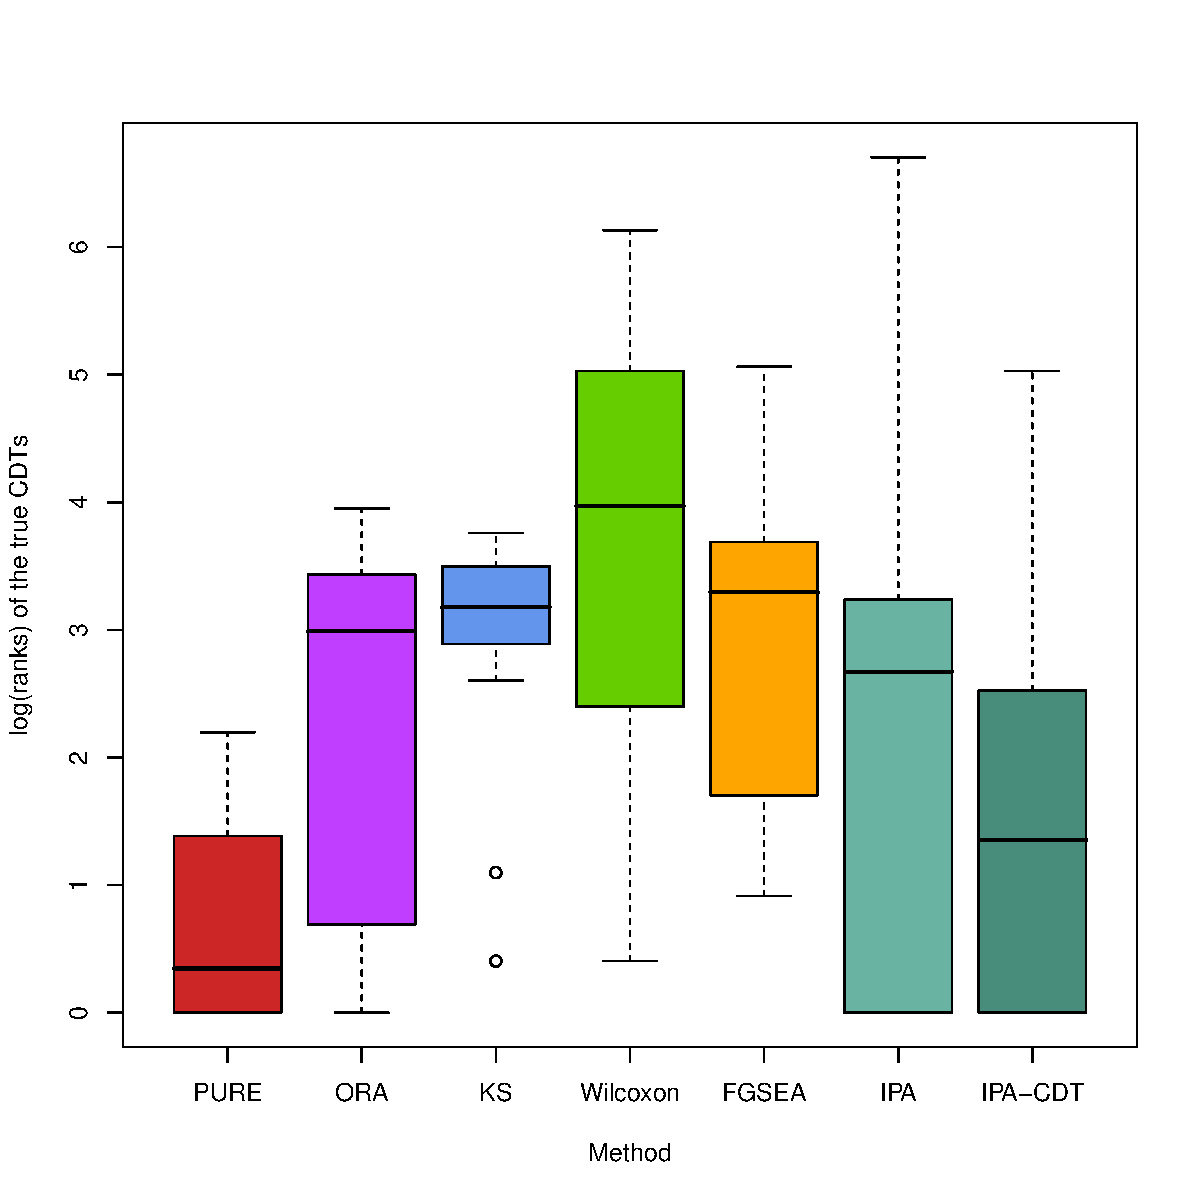
\includegraphics[width=0.49\linewidth]{Figures/RankTarget_vOrg_log.pdf}
%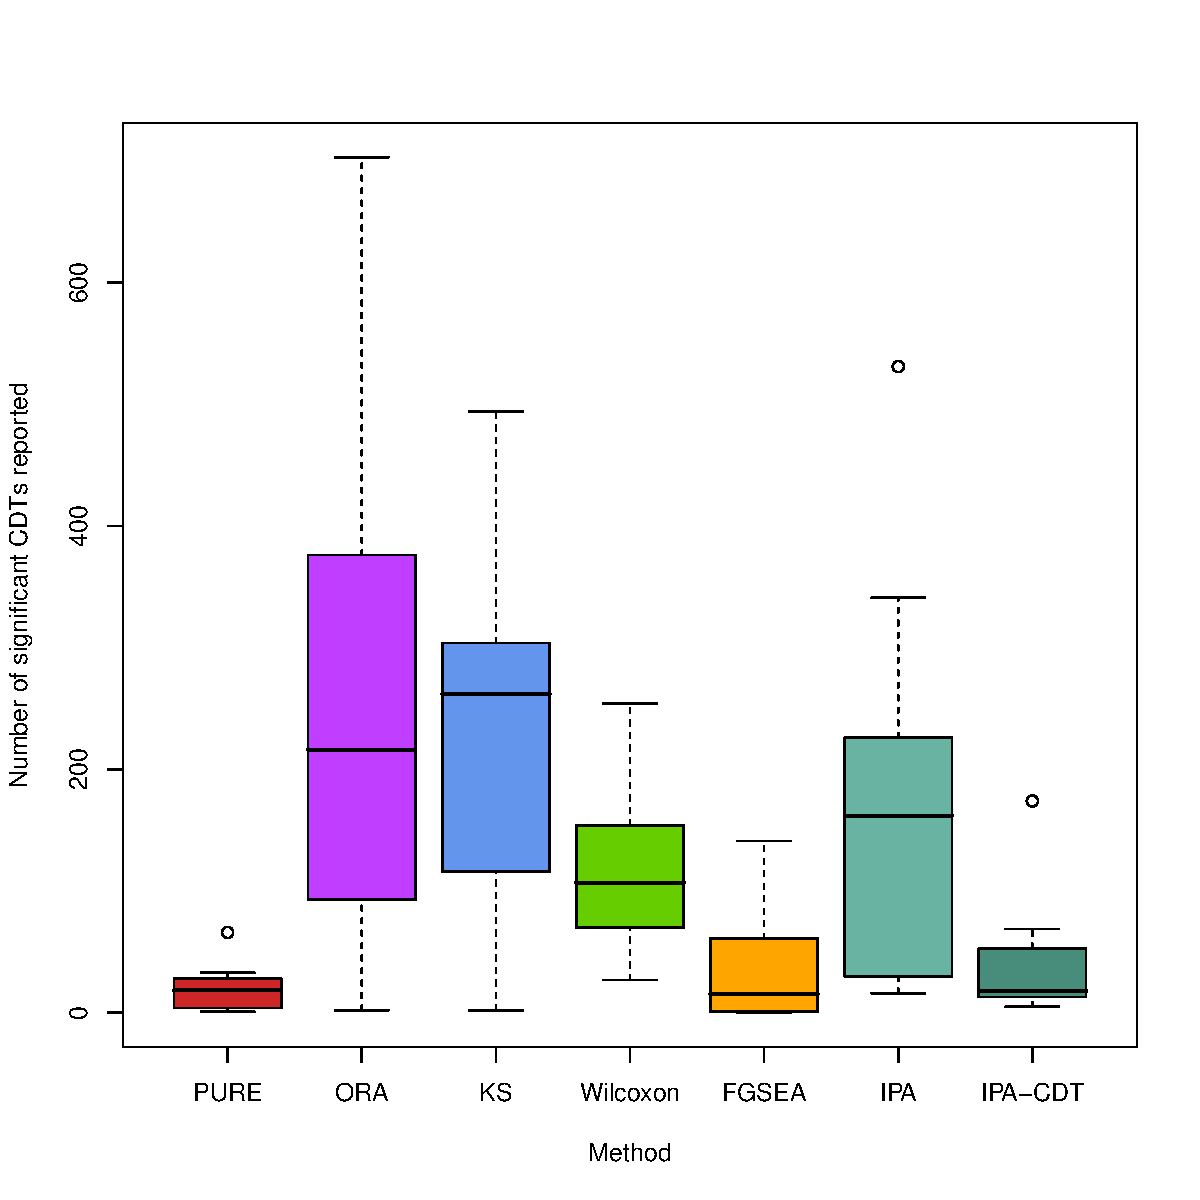
\includegraphics[width=0.49\linewidth]{Figures/NrSigChem_vOrg.pdf}
%%\includegraphics[width=0.32\linewidth]{Figures/pValueTarget_v2.pdf}
%
%\caption{The comparison of PURE and other 5 methods, in term of log(ranks) of true CDTs (left panel) and the number of significant chemicals reported (right panel). In the left panel, a better method would rank the true CDT as low as possible (ideally rank it 1) so lower log(rank) values are better. A CDT that is different from the true CDT and yet reported as significant is a false positive. For this reason, we would like the number of CDTs reported as significant (shown in the right panel) to also be as low as possible. }
%\label{fig:resultFigure}
%\end{center}
%\end{figure*}


\textbf{Definition of success}

To investigate whether the proposed method  is significantly superior to the other methods in term of testing the H1, we would use a Wilcoxon test to compare the ranks and number of CDTs reported by PURE with those provided by the  other methods. 
%The p values for the rank comparison of PURE and IPA-CDT, ORA, KS, FGSEA, IPA, and Wilcoxon are 0.02, 4E-4, 8E-6, 4E-5, 6E-3, and 1E-5, respectively. 
If the rank of the true CDTs is not available in an experiment, we replace the NA ranks by the number of significant CDTs reported in the corresponding experiment plus one, 
e.g. if a method reports a list of 30 significant CDTs but the true CDTs is not included, we assigned 31 to the true CDT's rank.
If the Wilcoxon p value is less than 5\%, we would conclude that the proposed method is statistically better at identifying the causal CDTs than other methods.

Regarding H2, we evaluate the methods' performance based on the same criteria: rank of the target CDT (Methylprednisolone), and the number of CDTs reported. 
%Our proposed method, PURE, is able to identify Methylprednisolone in both experiments with the average rank of 3.25, followed by FGSEA (average = 6.5), ORA (average = 14.75), KS (average = 19.5), Wilcoxon (average = 29), IPA-CDT (average = 393), and IPA (average = 890). Notice that although ORA, KS, Wilcoxon, and FGSEA can identify Methylprednisolone as significant CDT, they cannot determine whether it is present or absent. Also, IPA cannot identify Methylprednisolone in either experiments. More importantly, all other methods, except for FGSEA, reported hundreds of significant CDTs in each experiment, which make it difficult for a researcher to identify a truly effective drug such as Methylprednisolone. Hence, in term of number of CDTs reported, PURE also performs better than other methods. The average number of CDTs reported by PURE is 10 CDTs, whereas that number of FGSEA, IPA-CDT, Wilcoxon, KS, IPA, ORA are 27.5, 103, 189, 216, 238, 553, respectively (Table~\ref{H2Result}). 
Since the sample size is small (only 2 experiments), we do not compute p values for these comparisons. The average of the ranks in these two experiments derived by the benchmarking methods would be directly compared to each other.

\subsection{Discussion}

Beside  benchmarking the studied methods using real data sets as described in previous subsection, in this subsection we  would also compare the differences in theory of our approach versus the other competitive methods.
Moreover, we would discuss how our method improves and addresses the shortcomings of the related methods mentioned in section \ref{chap:ExisingMethodsLimitation} and its differences to other methods in the field. 

Among all the benchmarking methods included in this study, only IPA takes the sign of CDTs - genes associations under consideration and can predict whether a significant CDTs is activated or inhibited (corresponding to H1 and H2), as our proposed method does, so a more detailed theoretical comparison is warranted.
Although IPA derives these two scores  described above for each CDT, the result is solely determined by the z-score: the regulator is determined as ``activated''  or ``inhibited'' if its z-score $\geq 2$ or $\leq -2$, respectively~\cite{kramer2013causal}. In other words, the statistic calculated from the data will determine the outcome. In contrast, our proposed method uses a more classical approach in which the hypotheses are formulated before hand, independently of the data as in a canonical hypothesis testing. Our proposed method  considers each hypothesis separately, and calculates a p-value that will indicate whether the null hypothesis can be rejected. 
For our proposed method, the null hypothesis is that ``CDT X has not had an impact on the measured gene expression changes" whereas the first research hypothesis is that ``CTD X was present and had an impact on the gene expression changes'' and the second, independent, research hypothesis is that ``CTD X was lacking and its absence had an impact on the gene expression changes''. 
The testing done in the proposed approach is more rigorous in terms of statistical testing, but such approach can potentially reject the null hypothesis for both research hypotheses which would be difficult to interpret from a biological perspective. In contrast, the approach used by IPA avoids such potentially ambiguous situations because the z-score can be either positive or negative but not both. The most important difference stemming from these two approaches is that our proposed method  can identify CDTs that can reverse the observed genes expression changes because it considers both sets of statistical hypothesis. This means that our proposed method can be used for drug repurposing - situations in which one is given a   gene expression profile associated with a given disease and the task is to identify a drug that could revert some of the changes. In contrast, IPA only considers the CDTs that are present and focuses whether they are ``activated'' or ``inhibited''. 
Another  difference worth mentioning between IPA and our proposed method  is that while our proposed method  considers and derives a p value corresponding to the hypothesis testing for every CDT in the knowledge base, IPA does not derive z-score for all CDT in the knowledge base. %For example, Methylprednisolone is in the IPA's knowledge base and has z-score in the experiment 15, but no z-score is reported in the experiment 16 (Table ~\ref{H2Result}).

In other cases, the methods using reference gene-expression profiles, such as cMap~\cite{lamb2007connectivity, lamb2006connectivity} , LINCS (http://www.lincscloud.org/l1000/), sscMap~\cite{zhang2009sscmap} or SAM \cite{sirota2011discovery}, compare the gene expression of all genes measured in a disease or drug exposure (called disease's gene signature and drug's gene signature, respectively) to identify pairs of drug-disease that have the opposite signature or pairs of drug-drug that have similar gene signature. The gene signatures are often obtained from few data sets. However, they do not take into consider the fact that insufficient number of data sets to get the gene signatures is problematic. Ein-Dor {et al.} proved  that some gene expression profiles from a same condition are often different and have very few in common~\cite{ein2005outcome}. Our method, on the other hand, only focuses on the given gene profile and would proposes the potential CDT or identify the causal CDT for this specific case. It does not depend on the quantity, quality and lab condition of other experiments used to create the gene signatures database. Moreover, the number of drugs and small-molecule perturbagens in these databases is often limited. For example, in cMAP and SAM, there are less than 200 drugs' signatures. This small amount of drug signature makes this approach impractical. For example, SAM could not identify any potential drug for almost half of the diseases in the database (47 diseases out of 100 diseases). In contrast, our method scans through more than 5,000 CDTs and hence, have more chance to find a potential alternative treatment, especially with new diseases emerging, such as COVID-19. The complexity of comparing all available pairs of drug-disease and drug-drug is $\mathcal{O}(n^2)$ making it cost ineffective on large scale. On the other hand, with a given condition, our methods will derive the result with a complexity of $\mathcal{O}(n)$. One of the biggest drawback of this approach is the limited explanatory power since it cannot interpret which exact genes and mechanisms are affected by the proposed alternative drugs. Our method can identify precisely which and how DE genes are impacted by the proposed drugs.

In comparison with methods that create network of human diseases and potential drugs, our method will provide a list of sorted CDTs according to their p values. One can pick the top few suggested drugs instead of having to verify all the drugs connected to the disease in the disease-drug network. Moreover, our method is also easier to maintain and update regularly since the only source of modification is the CTD database. However, one must re-construct the network of hundred of diseases and drugs once there is any update in the knowledge base.
%
%Our method also utilizes the information of the interactions between drugs and downstream genes, compared to the classical gene set analysis methods.



